% TeX encoding = utf8
% TeX spellcheck = pl_PL 
\documentclass[a4paper, 12pt]{article}
\usepackage[utf8]{inputenc}
\usepackage[polish]{babel}
\usepackage{polski}
\usepackage{float}
\usepackage{graphicx}
\usepackage{listings}
\usepackage{amsfonts}
\usepackage{geometry}
\usepackage{indentfirst}
\usepackage{subfigure}
\usepackage{url}
\usepackage{listings}
\usepackage{color}
\usepackage{multicol}
\usepackage[usenames,dvipsnames]{xcolor}

%\renewcommand*{\addcontentsline}[3]{\addtocontents{#1}{\protect\contentsline{#2}{#3}{}}}
\newgeometry{tmargin=2.5cm, bmargin=2.5cm, lmargin=3.5cm, rmargin=2.5cm}
%\setcounter{secnumdepth}{2}
\setlength{\fboxsep}{0pt}
\lstset{
	basicstyle=\footnotesize\ttfamily,
	breaklines=true,
	language=Python,
	breakatwhitespace=true,
	frame=leftline,
	numbers=left,
	numberstyle=\tiny,
	commentstyle=\color{Gray}\footnotesize\ttfamily}


\author{Łukasz Korpal \\ Wiktor Ślęczka}
\title{Wyznaczanie w grafie najkrótszej ścieżki z ograniczoną liczbą krawędzi}


\begin{document}
	\sloppy
	\maketitle
	\newpage
	\tableofcontents
	\newpage
	\section{Realizowane zadanie}
	Dany jest spójny graf nieskierowany z określonymi długościami krawędzi i dwoma wyróżnionymi wierzchołkami. Problem polega na znalezieniu najkrótszej ścieżki między tymi wierzchołkami, składającej się z co najwyżej k krawędzi. W ramach projektu należy opracować algorytm i program do wyznaczania takiej ścieżki dla zadanego parametru k.
	
	\section{Interfejs programu}
	Utworzony w ramach projektu program należy uruchomić poprzez wydanie następującego polecenia:
	\begin{verbatim}
	gis <graph_description_file> <start> <target>
	\end{verbatim}
	Spowoduje to wczytanie podanego pliku, uruchomienie dla zapisanego w jego wnętrzu grafu algorytmu znajdowania ścieżki i wypisania znalezionego rozwiązania, lub komunikatu o napotkanym problemie. Dodatkowo muszą zostać podane wierzchołki startowy i końcowy oraz parametr określający maksymalną liczbę krawędzi, z których składać ma się ścieżka.
	\section{Założenia programu}
	Założenia dotyczą danych wejściowych. Są one następujące:
	\begin{itemize}
		\item Wierzchołek początkowy i końcowy muszą należeć do grafu
		\item Wierzchołek początkowy i końcowy każdej krawędzi są różne
		\item Minimalna liczba skoków jest całkowita dodatnia
		\item Podawany graf powinien być spójny i niekierowany
		\item Każda krawędź powinna mieć wagę
		\item Każdy wierzchołek powinien mieć unikalną nazwę
		\item Krawędź łączy zdefiniowane uprzednio wierzchołki
		\item Wagi krawędzi muszą mieć wartości dodatnie całkowite
		\item Dla metody BFS między dwoma dowolnymi wierzchołkami nie powinno być więcej niż jednej krawędzi
		\item Pliki wejściowe są stworzone zgodnie z podaną specyfikacją
	\end{itemize}
	
	\section{Wejście}
	Wejściem programu jest pojedynczy plik tekstowy, zawierający opis grafu.
	Na jego początku znajduje się lista wierzchołków, oddzielonych znakiem nowej linii. W nazwie wierzchołka mogą znaleźć się dowolne znaki nie będące znakami białymi.
	Pierwsza linia pliku zawiera informacje o wielkości grafu:
	\begin{verbatim}
	<liczba_wierzchołków> <liczba_krawedzi>
	\end{verbatim}
	Następnie podawana jest lista krawędzi, gdzie krawędź jest zdefiniowana jako
	\begin{verbatim}
	<nazwa_wierzchołka_1> <nazwa_wierzchołka_2> <waga_krawedzi>
	\end{verbatim}
	definiująca po jednej krawędzi w każdej kolejnej linii.
	Na końcu pliku występuje pojedyncza pusta linia.
	
	
	\section{Wyjście}
	Wyjściem programu jest lista wierzchołków, na które składa się znaleziona ścieżka, wraz z jej obliczoną długością. Wierzchołki rozpoznawane są poprzez nazwy podane w pliku opisującym graf.
	
	\section{Technologie} 
	\subsection{Projekt}
	Projekt jest realizowany przy użyciu języka Scala w wersji 2.11.8. W chwili obecnej nie są wykorzystywane żadne dodatkowe biblioteki ani innego rodzaju zależności. Do kompilacji programu używane jest narzędzie SBT.
	\subsection{Testy}
	Grafy tworzone są na potrzeby testów przy użyciu skryptu języka Python, korzystającego z biblioteki GraphViz, służącej ich wizualizacji.
	\section{Struktury danych}
	W programie będą wykorzystywane dwie struktury danych: jedna odpowiedzialna za przechowywanie grafu wczytanego z pliku tekstowego oraz druga, przechowująca aktualny stan procesu przeszukiwania grafu.
	Klasa opisująca obiekt wczytanego grafu będzie składała się z dwóch list, reprezentujących wierzchołki i krawędzie. Instancja wierzchołka pozwala na sprawdzenie krawędzi, które z niego wychodzą, natomiast krawędzi sprawdza, czy wierzchołek jest do niej przyłączony.
	Konstruktor pozwala na utworzenie pustego grafu, który będzie zapełniany w miarę odczytywania informacji z pliku w trakcie inicjalizacji programu.
	
	Aktualny stan procesu przeszukiwania grafu reprezentowany będzie przez mapę przypisującą do każdego wierzchołka odległość od punktu startowego oraz inne, niezbędne do przeszukiwania informacje, pozwalające odtworzyć ścieżkę prowadzącą do opisywanego wierzchołka.
	Mapa realizowana będzie poprzez wbudowany typ mapy.
	
	\section{Wykorzystane algorytmy}
	Algorytm wykorzystywany do odnajdywania najlżejszej ścieżki w grafie będzie algorytm bazujący na algorytmie DFS. Jego działanie opiera się na sprawdzaniu wierzchołków o najkrótszej długości drogi (do maksymalnej liczby skoków) do momentu dotarcia do wierzchołka docelowego.
	W przypadku sprawdzania wierzchołków oddalonych o więcej niż maksymalną liczbę skoków, algorytm pomija takie rozwiązanie i wyszukuje kolejnych możliwości poprawy ścieżki.
	W przypadku, gdy podczas tworzenia grafu wykryte zostanie, że wszystkie krawędzie są takiej samej długości, zastosowany zostanie inny algorytm, przyspieszający rozwiązanie zadania. Algorytmem tym będzie Breadth First Search.
	\subsection{Algorytm przedstawiony w pseudokodzie}
	\begin{verbatim}
DFS(from, to, maxjumps, distance=0):
  if maxjumps == 0:
    return routes
  for each neighbour from.neighbours:
    DFS(neighbour, to, maxjumps-1, distance+dist(from, neighbour))
  if from == to && (routes is empty || routes.distance > distance):
    routes.change(from,distance)  			
	\end{verbatim}
	
	\section{Testy}
	Testy programu zostały przeprowadzone zarówno dla grafów tworzonych losowo, jak i specjalnie przygotowanych przypadków szczególnych.
	\subsection{Przypadki szczególne}
	\begin{figure}
			\subfigure[Przypadek tworzący linię prostą.]{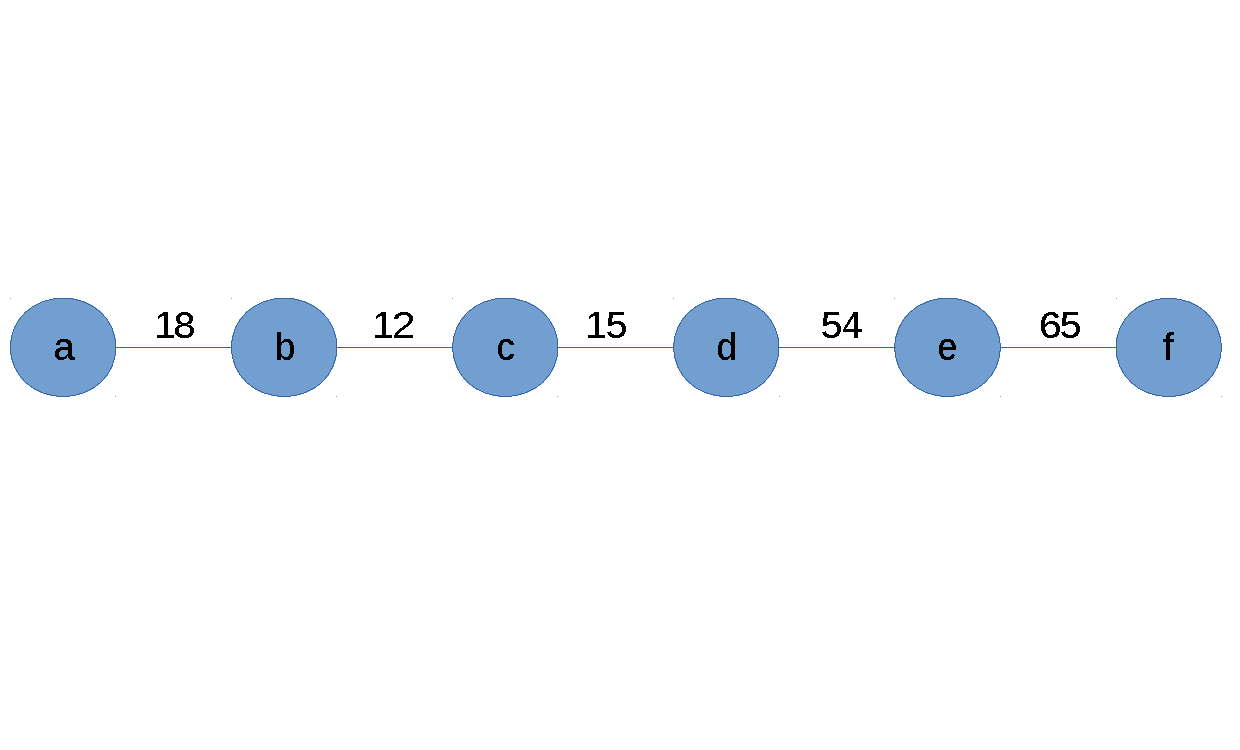
\includegraphics[width=0.5\columnwidth]{testy/prosta.pdf}}
			\label{prosta}
			\subfigure[Przypadek sprawdzający poprawne działanie wyboru najkrótszej drogi.]{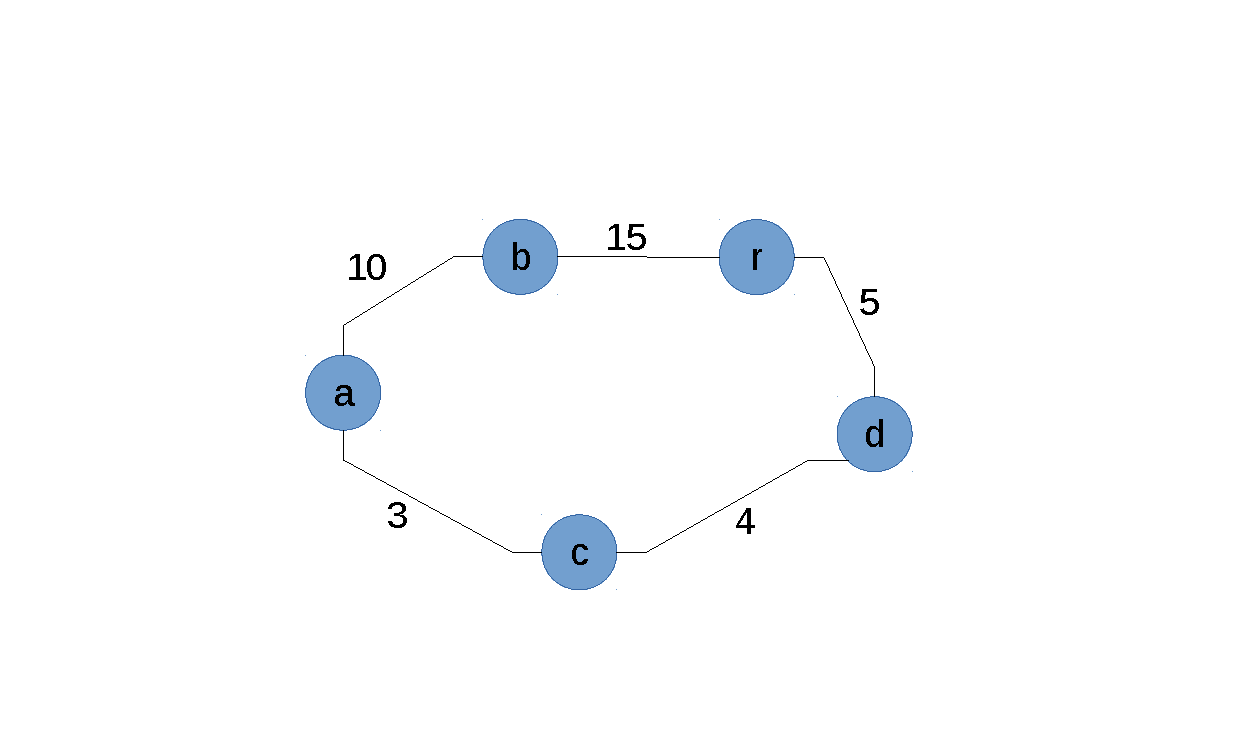
\includegraphics[width=0.5\columnwidth]{testy/kolo.pdf}}
			\label{kolo}
			\subfigure[[Przypadek tworzący linię prostą, uruchamiający przeszukiwanie BFS.]{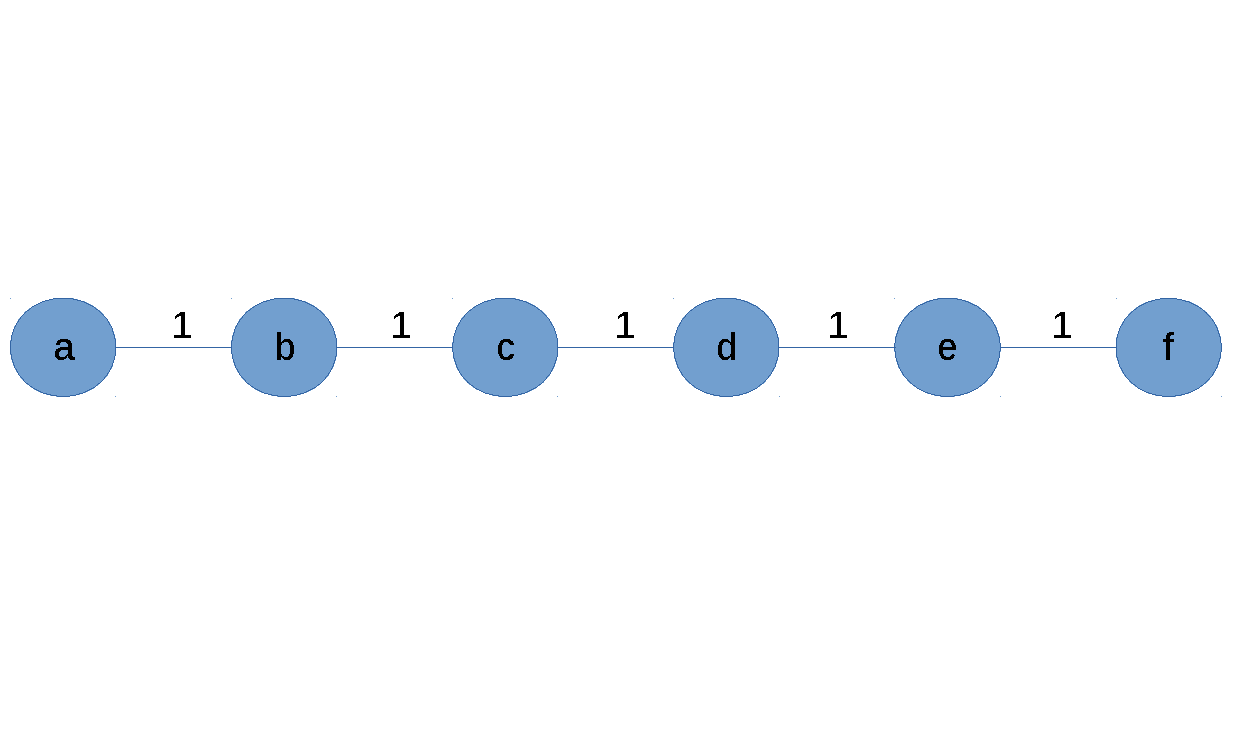
\includegraphics[width=0.5\columnwidth]{testy/prosta_BFS.pdf}}
			\label{prostaBFS}
			\caption{Przypadki szczególne}
	\end{figure}
	
	\subsection{Grafy tworzone losowo}
	Grafy tworzone były za pomocą skryptu $creator\_viz.py$
	\begin{figure}
			\subfigure[Przypadek, w którym graf uruchamia metodę BFS.]{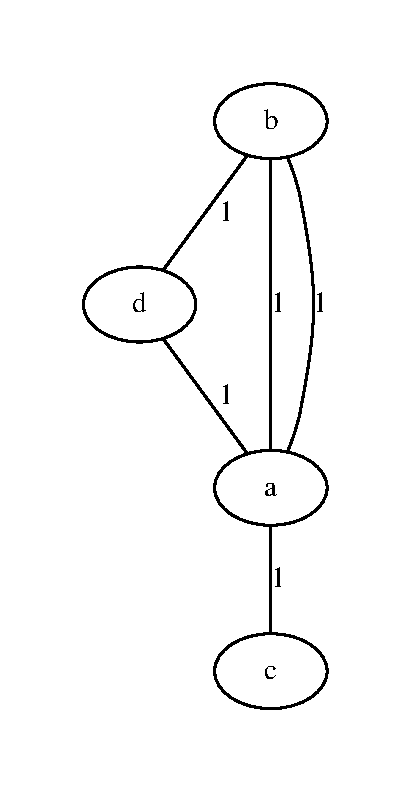
\includegraphics[width=0.5\columnwidth]{testy/BFS.pdf}}
			\label{BFS}
			\subfigure[Przypadek dla 4 wierzchołków i 5 krawędzi.]{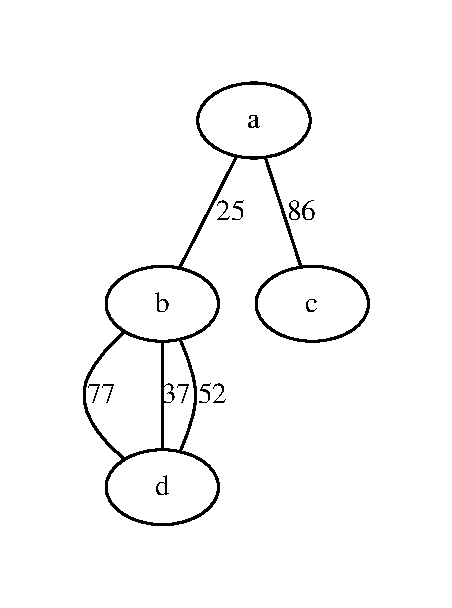
\includegraphics[width=0.5\columnwidth]{testy/4_5.pdf}}
			\label{4_5}
			\subfigure[Przypadek dla 5 wierzchołków i 10 krawędzi.]{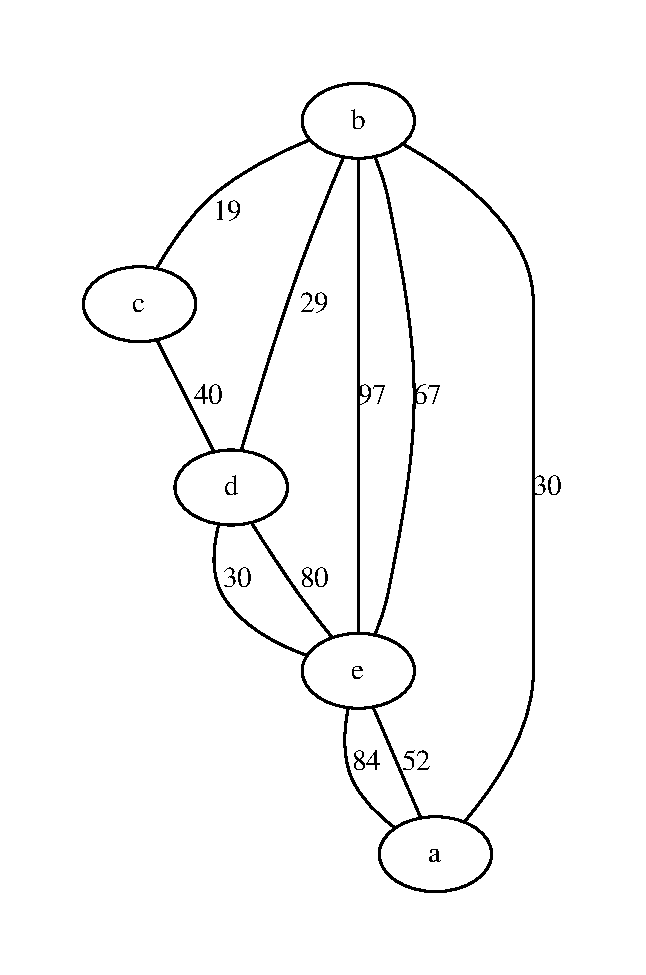
\includegraphics[width=0.5\columnwidth]{testy/5_10.pdf}}
			\label{5_10}
			\caption{Grafy tworzone losowo - część 1}		
\end{figure}
\begin{figure}
	\centering
			\subfigure[Przypadek dla 7 wierzchołków i 20 krawędzi.]{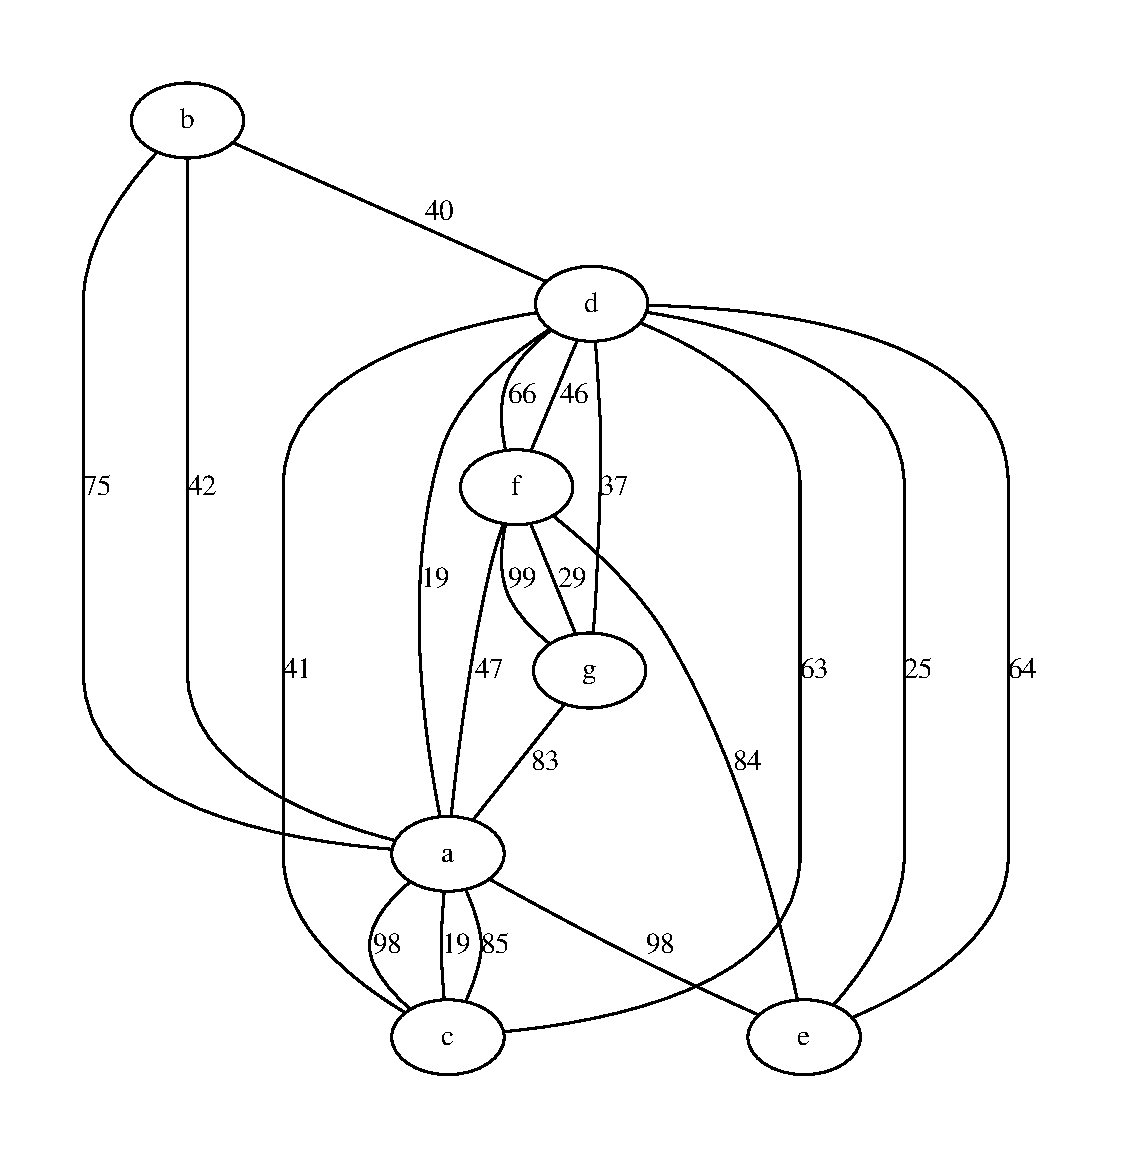
\includegraphics[width=0.5\columnwidth]{testy/7_20.pdf}}
			\label{7_20}
			\subfigure[Przypadek dla 14 wierzchołków i 50 krawędzi.]{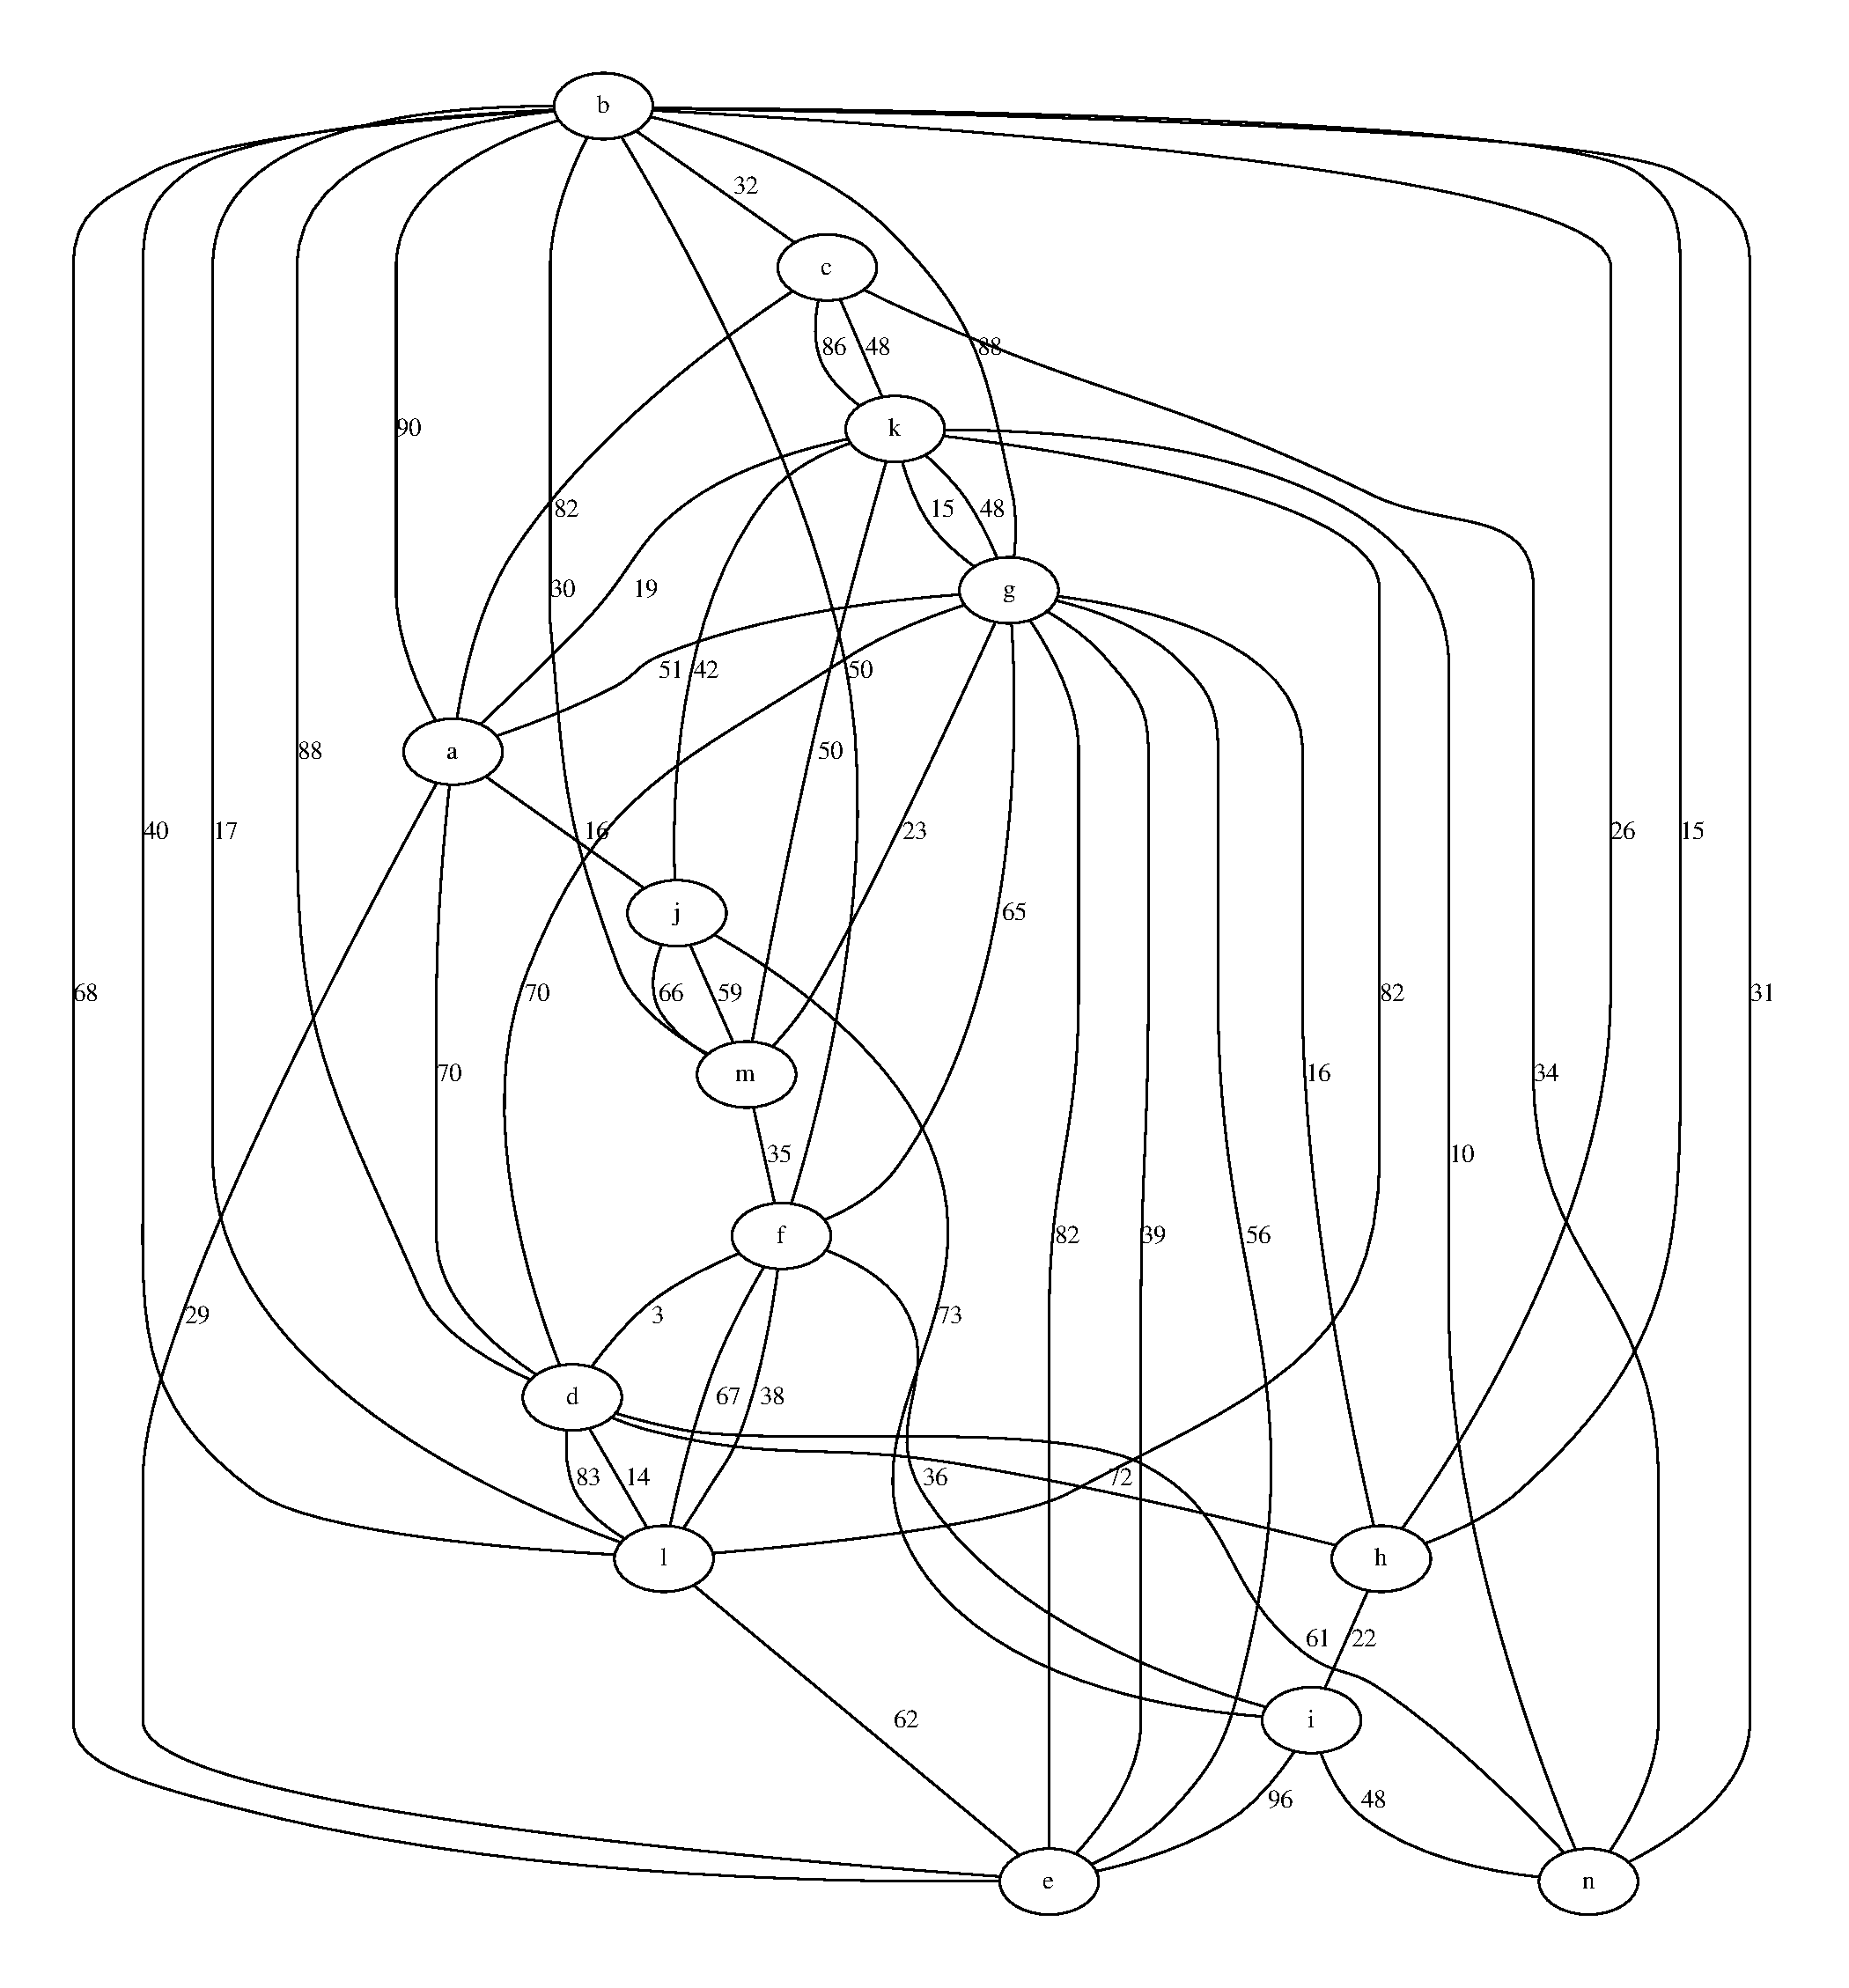
\includegraphics[width=0.8\columnwidth]{testy/14_50.pdf}}
			\label{14_50}
			\caption{Grafy tworzone losowo - część 2}
\end{figure}
	
\section{Wyniki}
Testy przeprowadzano na komputerze z procesorem AMD Phenom(tm) II X6 1090T. Około 0.4 sekundy z podanych czasów jest pochłaniane na uruchamianie wirtualnej maszyny Java.\\
Dla podanych przykładów wyniki działania programu, poszukującego ścieżki - dla ograniczenia do odległości 5 krawędzi - były następujące:
\begin{itemize}

    \begin{multicols}{2}
\item \ref{prosta} a \begin{verbatim}
Distance: 99
a
b
c
d
e
\end{verbatim}
Czas wykonania: 0m0.399s
\item \ref{kolo} b \begin{verbatim}
Distance: 12
a
c
d
e
\end{verbatim}
Czas wykonania: 0m0.383s
\item \ref{prostaBFS} c \begin{verbatim}
Distance: 5
a
b
c
d
e
f
\end{verbatim}
Czas wykonania: 0m0.659s
\item \ref{BFS} a \begin{verbatim}
Distance: 2
c
a
b
\end{verbatim}
Czas wykonania: 0m0.544s
\item \ref{4_5} b \begin{verbatim}
Distance: 86
a
c
\end{verbatim}
Czas wykonania: 0m0.354s
\item \ref{5_10} c \begin{verbatim}
Distance: 49
a
b
c
\end{verbatim}
Czas wykonania: 0m0.375s
\item \ref{7_20} a \begin{verbatim}
Distance: 56
a
d
g
\end{verbatim}
Czas wykonania: 0m0.433s
\item \ref{14_50} b \begin{verbatim}
Distance: 50
a
k
g
h
\end{verbatim}
Czas wykonania: 0m0.580s
  \end{multicols}
\end{itemize}
Dla największego testowanego grafu (12000 wierzchołków i 50000 krawędzi)
\begin{verbatim}
Distance: 265
ax
oxa
qku
coh
bun
abs
\end{verbatim}
Czas wykonania dla maksymalnej liczby skoków:\\
6 0m32.022s\\ 
7 0m43.391s\\
8 1m22.649s\\

Dla innego wygenerowanego grafu zawierającego tyle samo krawędzi i wierzchołków, jednak rozpatrywanego algorytmem BFS (tworzone wagi krawędzi są równe 1) wynik jest następujący:
\begin{multicols}{2}
\begin{verbatim}
Distance: 41
ax
hyr
pxm
b
ihe
bum
ojk
dfz
puh
dwj
csn
mef
acz
jbv
pkb
itu
dqe
gsq
fft
erk
gdo
ivw
cqz
qfv
cey
dmo
apc
pyh
mg
ckz
nfq
jbg
jpf
frk
rx
avh
axr
cna
dxw
jko
uw
abs
\end{verbatim}
\end{multicols}
Czas wykonania: 0m2.744s
\section{Wnioski}
Oryginalny algorytm DFS, zmodyfikowany o skracanie poszukiwań do maksymalnej odległości (wyrażonej w skokach) sprawdza się bardzo dobrze dla ilości wierzchołków poniżej rzędu wielkości $2 \cdot 10^4$ i ilości krawędzi poniżej $10^5$.
Dla wartości liczby wierzchołków zbliżających się do tej granicy czas oczekiwania na wynik działania programu trwa ponad 3 minuty (przy pełnym użyciu procesora Intel Core i5 o taktowaniu 2.4 GHz).\\
Porównanie działania algorytmów BFS i zmodyfikowanego algorytmu DFS wyraźnie pokazują, że dla dużych grafów algorytm BFS działa nieporównywalnie sprawniej.

\end{document}


